\documentclass{article}

% content/resources/templates/preamble.tex
\usepackage[margin=0.6in]{geometry}
\author{Milav Dabgar}
\usepackage{amsmath,amssymb,amsthm}
\usepackage{booktabs}
\usepackage{multirow}
\usepackage{xcolor}
\usepackage{tcolorbox}
\tcbuselibrary{breakable,skins}
\usepackage[colorlinks=true,linkcolor=blue]{hyperref}
\usepackage{titlesec}
\usepackage{enumitem}
\usepackage{tikz}
\usepackage{pgfplots}
\usepackage{circuitikz}
\usepackage[version=4]{mhchem}
\usepackage{longtable}
\usepackage{array}
\usepackage{float}
\usepackage{caption}
\usepackage{listings}

\lstset{
  basicstyle=\small\ttfamily,
  breaklines=true,
  breakatwhitespace=false,
  postbreak=\mbox{\textcolor{red}{$\hookrightarrow$}\space},
  float=false,
  numbers=left,
  numberstyle=\tiny\color{gray},
  numbersep=10pt,
  xleftmargin=2em,
  keywordstyle=\color{blue},
  commentstyle=\color{green!60!black},
  stringstyle=\color{purple},
  backgroundcolor=\color{gray!5},
  showstringspaces=false,
  tabsize=2,
  captionpos=b,
  keepspaces=true,
  columns=flexible
}

\pgfplotsset{compat=1.18}
\usetikzlibrary{shapes,arrows,positioning,calc,patterns,decorations.pathmorphing,decorations.markings,arrows.meta}

% Color scheme
\definecolor{headcolor}{RGB}{0,102,204}
\definecolor{keycolor}{RGB}{220,20,60}
\definecolor{solutioncolor}{RGB}{34,139,34}
\definecolor{mnemoniccolor}{RGB}{148,0,211}
\definecolor{codecolor}{RGB}{0,0,100}

% Spacing
\setlength{\parskip}{3pt}
\setlist[itemize]{nosep}
\setlist[enumerate]{nosep}

% Title formatting
\titleformat{\section}{\Large\bfseries\color{headcolor}}{\thesection}{1em}{}
\titleformat{\subsection}{\large\bfseries\color{headcolor}}{\thesubsection}{1em}{}

% Pandoc tightlist compatibility
\providecommand{\tightlist}{%
  \setlength{\itemsep}{0pt}\setlength{\parskip}{0pt}}

% Pandoc longtable compatibility
\newcounter{none}
\def\thenone{}


% content/resources/templates/english-boxes.tex

% Custom environments
\newtcolorbox{solutionbox}{
 breakable,
 enhanced,
 colback=solutioncolor!5!white,
 colframe=solutioncolor!75!black,
 fonttitle=\bfseries,
 title=Solution
}

\newtcolorbox{solutionboxnobreak}{
 colback=solutioncolor!5!white,
 colframe=solutioncolor!75!black,
 fonttitle=\bfseries,
 title=Solution
}

\newtcolorbox{keyformula}{
 breakable,
 enhanced,
 colback=keycolor!5!white,
 colframe=keycolor!75!black,
 fonttitle=\bfseries,
 title=Key Formula
}

\newtcolorbox{mnemonicboxenv}{
 breakable,
 enhanced,
 colback=mnemoniccolor!5!white,
 colframe=mnemoniccolor!75!black,
 fonttitle=\bfseries,
 title=Mnemonic
}

\newcommand{\mnemonicbox}[1]{%
  \begin{mnemonicboxenv}
    #1
  \end{mnemonicboxenv}
}


% Custom commands for GTU solutions
% This file defines semantic commands for consistent formatting

% Question command with automatic formatting
\newcommand{\question}[2]{%
  \section*{Question #1}%
  \textbf{#2}%
}

% OR question variant
\newcommand{\questionor}[2]{%
  \section*{Question #1 OR}%
  \textbf{#2}%
}

% Proper table environment with caption
\newenvironment{answertable}[1]{%
  \begin{table}[htbp]
  \centering
  \caption{#1}
}{%
  \end{table}
}

% Proper figure environment for diagrams
\newenvironment{answerdiagram}[1]{%
  \begin{figure}[htbp]
  \centering
  \caption{#1}
}{%
  \end{figure}
}

% Semantic markup for key terms
\newcommand{\keyword}[1]{\textbf{#1}}
\newcommand{\code}[1]{\texttt{#1}}
\newcommand{\classname}[1]{\texttt{#1}}
\newcommand{\methodname}[1]{\texttt{#1}}

% Proper quotation marks
\newcommand{\mnemonic}[1]{``#1''}


\title{Electronic Measurements and Instruments (4331102) - Summer 2023 Solution}
\date{July 19, 2023}

\begin{document}
\maketitle

\questionmarks{1(a)}{3}{Illustrate steps to minimize that all type of systematic error.}

\begin{solutionbox}
\textbf{Steps to minimize systematic errors:}
\begin{center}
\captionof{table}{Steps to Minimize Systematic Errors}
\begin{tabulary}{\linewidth}{|L|L|}
\hline
\textbf{Step} & \textbf{Description} \\ \hline
\textbf{1. Calibration} & Periodically calibrate instruments against standard references \\ \hline
\textbf{2. Correction} & Apply correction factors or offset values \\ \hline
\textbf{3. Control} & Maintain constant environmental conditions (temperature, humidity) \\ \hline
\textbf{4. Technique} & Use proper measurement techniques and procedures \\ \hline
\textbf{5. Equipment} & Select appropriate instruments with required accuracy \\ \hline
\end{tabulary}
\end{center}
\end{solutionbox}

\begin{mnemonicbox}
\mnemonic{CCCTS: Calibrate, Correct, Control, Technique, Select}
\end{mnemonicbox}

\questionmarks{1(b)}{4}{Define: Resolution, Precision, Sensitivity and Accuracy.}

\begin{solutionbox}
\begin{center}
\captionof{table}{Measurement Characteristics Definitions}
\begin{tabulary}{\linewidth}{|L|L|}
\hline
\textbf{Term} & \textbf{Definition} \\ \hline
\textbf{Resolution} & The smallest change in input that can be detected by the instrument \\ \hline
\textbf{Precision} & Consistency or repeatability of measurements with minimal random error \\ \hline
\textbf{Sensitivity} & The ratio of change in output to the change in input ($\Delta O/\Delta I$) \\ \hline
\textbf{Accuracy} & Closeness of measured value to the true or accepted standard value \\ \hline
\end{tabulary}
\end{center}

\begin{center}
\begin{circuitikz}[
    level 1/.style = {sibling distance=4cm},
    level 2/.style = {sibling distance=2.5cm},
    edge from parent/.style = {draw, -latex},
    every node/.style = {rectangle, draw, rounded corners, align=center, font=\small}
]
    \node {Measurement Quality}
        child { node {Resolution}
            child { node {Smallest Change} }
        }
        child { node {Precision}
            child { node {Repeatability} }
        }
        child { node {Sensitivity}
            child { node {Output/Input} }
        }
        child { node {Accuracy}
            child { node {Closeness to Truth} }
        };
\end{circuitikz}
\captionof{figure}{Measurement Characteristics}
\end{center}
\end{solutionbox}

\begin{mnemonicbox}
\mnemonic{RSPA: Resolve Signals Precisely and Accurately}
\end{mnemonicbox}

\questionmarks{1(c)}{7}{Explain a principle of Q Meter and Working of practical Q Meter.}

\begin{solutionbox}
\textbf{Principle:}
\begin{itemize}
    \item Based on series resonance where $Q = X_L/R$ or $X_C/R$ at resonance
    \item Measures voltage magnification at resonance condition
\end{itemize}

\textbf{Working of practical Q meter:}
\begin{center}
\captionof{table}{Components of Practical Q Meter}
\begin{tabulary}{\linewidth}{|L|L|}
\hline
\textbf{Component} & \textbf{Function} \\ \hline
\textbf{Oscillator} & Generates variable frequency signal (50kHz to 50MHz) \\ \hline
\textbf{Work coil} & Inductor under test (connected in series with calibrated capacitor) \\ \hline
\textbf{Capacitor} & Variable calibrated capacitor for resonance tuning \\ \hline
\textbf{VTVM} & Measures resonant voltage across capacitor \\ \hline
\textbf{Shunt resistor} & Monitors current through the circuit \\ \hline
\end{tabulary}
\end{center}

\begin{center}
\begin{circuitikz}[auto]
    \draw (0,0) to [sV, l=RF Source] (0,2) -- (2,2) coordinate (A);
    \draw (A) to [L, l=$L_x$ (Work Coil)] (4,2) coordinate (B);
    \draw (B) to [vC, l=$C$ (Tuning)] (4,0) coordinate (C);
    \draw (C) -- (0,0);
    
    \draw (B) -- (6,2) coordinate (Vtop);
    \draw (C) -- (6,0) coordinate (Vbot);
    \draw (Vtop) to [voltmeter, l=VTVM (Q Reading)] (Vbot);
    
    \draw (0,0) to [R, l=$R_{sh}$] (2,0); % Series injection Rsh usually in osc path, simplified here
\end{circuitikz}
\captionof{figure}{Practical Q Meter}
\end{center}

\begin{itemize}
    \item \textbf{Q factor calculation}: $Q = V_2/V_1$ where $V_2$ is voltage across capacitor and $V_1$ is the applied voltage
    \item \textbf{Resonance indication}: Maximum voltage across capacitor indicates resonance
\end{itemize}
\end{solutionbox}

\begin{mnemonicbox}
\mnemonic{VOCAL: Voltage ratio at resonance Oscillator Creates Amplification to measure coiL quality}
\end{mnemonicbox}

\questionmarks{1(c OR)}{7}{Explain Wheatstone bridge and derive equation for balanced condition. State application and limitation of Wheatstone bridge.}

\begin{solutionbox}
Wheatstone bridge is a network used to measure unknown resistance with high precision.

\begin{center}
\begin{circuitikz}[auto]
    \draw (0,3) coordinate (A) -- (2,4) coordinate (D) -- (4,3) coordinate (C) -- (2,2) coordinate (B) -- (A);
    \draw (A) -- (-1,3); \draw (C) -- (5,3); % Terminals
    
    \node [above] at (D) {D}; \node [below] at (B) {B};
    \node [left] at (A) {A}; \node [right] at (C) {C};
    
    \path (A) -- (D) node[midway, above left] {$R_1$};
    \path (D) -- (C) node[midway, above right] {$R_x$ (Unknown)};
    \path (A) -- (B) node[midway, below left] {$R_2$};
    \path (B) -- (C) node[midway, below right] {$R_3$};
    
    \draw (D) to [ammeter, l=G] (B);
    
    \draw (-1,3) to [battery1, l=E] (-1,1) -| (2,1) -- (B); % Simplified source connection
    \draw (2,1) -- (2,0.5) node[ground]{}; % Optional ground
\end{circuitikz}
\captionof{figure}{Wheatstone Bridge}
\end{center}

\textbf{Balanced Condition Derivation:}
\begin{itemize}
    \item At balance, no current flows through galvanometer ($I_G = 0$)
    \item Potential at point D = Potential at point B
    \item Voltage drop across $R_1$ = Voltage drop across $R_2$ ($I_1 R_1 = I_2 R_2$)
    \item Voltage drop across $R_x$ = Voltage drop across $R_3$ ($I_1 R_x = I_2 R_3$)
\end{itemize}
Dividing the equations:
\[ \frac{I_1 R_1}{I_1 R_x} = \frac{I_2 R_2}{I_2 R_3} \implies \frac{R_1}{R_x} = \frac{R_2}{R_3} \implies R_x = R_3 \left( \frac{R_1}{R_2} \right) \]

\textbf{Applications \& Limitations:}
\begin{center}
\captionof{table}{Wheatstone Bridge Applications and Limitations}
\begin{tabulary}{\linewidth}{|L|L|}
\hline
\textbf{Application} & \textbf{Limitation} \\ \hline
Precision resistance measurement & Poor accuracy for low resistances ($<1\Omega$) \\ \hline
Transducer interface (Strain gauge, RTD) & Limited by galvanometer sensitivity \\ \hline
Temperature measurement & Contact resistance affects accuracy \\ \hline
\end{tabulary}
\end{center}
\end{solutionbox}

\begin{mnemonicbox}
\mnemonic{BEAR: Balance Equation at Arms Ratio}
\end{mnemonicbox}

% ==================================================================
% QUESTION 2
% ==================================================================

\questionmarks{2(a)}{3}{Differentiate between moving iron and moving coil type instruments.}

\begin{solutionbox}
\begin{center}
\captionof{table}{Comparison: Moving Iron vs PMMC Instruments}
\begin{tabulary}{\linewidth}{|L|L|L|}
\hline
\textbf{Parameter} & \textbf{Moving Iron (MI)} & \textbf{Moving Coil (PMMC)} \\ \hline
\textbf{Principle} & Magnetic attraction/repulsion & EM force on conductor \\ \hline
\textbf{Scale} & Non-uniform (crowded at start) & Uniform (linear) \\ \hline
\textbf{Supply} & AC and DC & DC only \\ \hline
\textbf{Accuracy} & Lower ($1-2.5\%$) & Higher ($0.1-1\%$) \\ \hline
\textbf{Damping} & Air friction & Eddy current \\ \hline
\textbf{Power} & Higher consumption & Lower consumption \\ \hline
\end{tabulary}
\end{center}
\end{solutionbox}

\begin{mnemonicbox}
\mnemonic{IRON-COIL: Iron Repulsion Non-uniform; Coil Current Linear}
\end{mnemonicbox}

\questionmarks{2(b)}{4}{Draw the construction diagram of clamp on Ammeter and explain in detail.}

\begin{solutionbox}
\textbf{Construction Diagram:}
\begin{center}
\begin{circuitikz}[auto]
    \draw (0,0) [rounded corners=0.5cm] -- (0,3) -- (3,3) -- (3,0) -- cycle; % Body
    \draw (0.5,3) [rounded corners=1cm] -- (0.5,5) -- (2.5,5) -- (2.5,3); % Clamp jaws
    \draw (0.5,3) -- (2.5,3); % Jaw base
    \draw [thick] (1.5,4) circle (0.2); \node at (1.5,4) {$\bullet$}; \node [right] at (1.7,4) {Conductor};
    
    \draw (0.5,2) rectangle (2.5,2.8); \node at (1.5,2.4) {Display};
    \draw (0.5,0.5) rectangle (2.5,1.5); \node at (1.5,1) {Controls};
    
    \node [left] at (0,4) {Jaws (CT Core)};
    \draw [->] (-0.5,4) -- (0.5,4.5);
\end{circuitikz}
\captionof{figure}{Clamp-on Ammeter}
\end{center}

\textbf{Working:}
\begin{itemize}
    \item \textbf{Transformer Principle}: The current-carrying conductor acts as a single-turn primary winding of a transformer.
    \item \textbf{Core \& Secondary}: The clamp jaws form the magnetic core required for flux path. A secondary winding inside the casing picks up the induced current.
    \item \textbf{Measurement}: The induced secondary current is proportional to the primary current, which is processed and displayed.
    \item \textbf{Non-intrusive}: Allows current measurement without breaking the circuit.
\end{itemize}
\end{solutionbox}

\begin{mnemonicbox}
\mnemonic{CLASP: Conductor-Loop Amperes Sensed by Primary-secondary}
\end{mnemonicbox}

\questionmarks{2(c)}{7}{Describe working and advantages of Integrating type DVM with suitable diagram.}

\begin{solutionbox}
Integrating DVM uses dual-slope integration to measure voltage, effectively canceling out noise.

\textbf{Block Diagram:}
\begin{center}
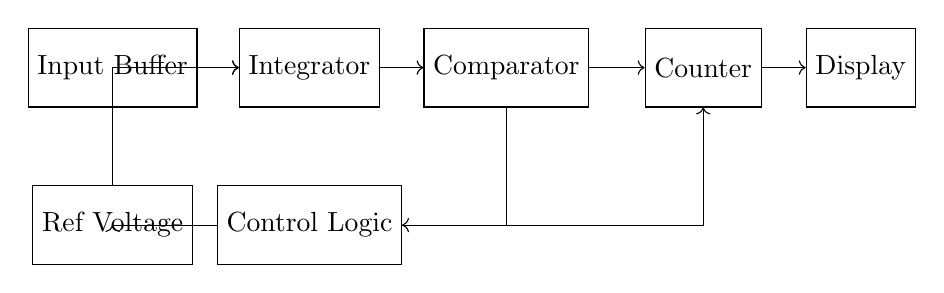
\begin{tikzpicture}[auto, node distance=2cm, every node/.style={draw, rectangle, minimum height=1cm, align=center}]
    \node (buf) {Input Buffer};
    \node [right of=buf, node distance=2.5cm] (int) {Integrator};
    \node [right of=int, node distance=2.5cm] (cmp) {Comparator};
    \node [right of=cmp, node distance=2.5cm] (cnt) {Counter};
    \node [right of=cnt, node distance=2cm] (disp) {Display};
    
    \node [below of=int] (log) {Control Logic};
    \node [left of=log, node distance=2.5cm] (ref) {Ref Voltage};
    
    \draw [->] (buf) -- (int);
    \draw [->] (int) -- (cmp);
    \draw [->] (cmp) -- (cnt);
    \draw [->] (cnt) -- (disp);
    
    \draw [->] (log) -| (ref);
    \draw [->] (ref) |- (int); % Switch conceptually
    \draw [->] (cmp) |- (log);
    \draw [->] (log) -| (cnt);
\end{tikzpicture}
\captionof{figure}{Integrating DVM}
\end{center}

\textbf{Working Principle:}
\begin{enumerate}
    \item \textbf{Run-up}: Unknown voltage $V_{in}$ charges the integrator capacitor for a fixed time period $T_1$.
    \item \textbf{Run-down}: A reference voltage $V_{ref}$ of opposite polarity discharges the capacitor until it reaches zero. Time taken is $T_2$.
    \item \textbf{Measurement}: Since charge up = charge down, $V_{in} T_1 = V_{ref} T_2 \implies V_{in} = V_{ref} \frac{T_2}{T_1}$.
\end{enumerate}

\textbf{Advantages:}
\begin{itemize}
    \item High noise rejection (esp. mains frequency).
    \item High accuracy and resolution.
    \item Good stability and linearity.
\end{itemize}
\end{solutionbox}

\begin{mnemonicbox}
\mnemonic{RISES: Ramp Integration Samples and Eliminates Spikes}
\end{mnemonicbox}

\questionmarks{2(a OR)}{3}{Differentiate between Digital Voltmeter over Analog Voltmeter.}

\begin{solutionbox}
\begin{center}
\captionof{table}{Comparison: Digital vs Analog Voltmeter}
\begin{tabulary}{\linewidth}{|L|L|L|}
\hline
\textbf{Parameter} & \textbf{Digital Voltmeter} & \textbf{Analog Voltmeter} \\ \hline
\textbf{Display} & Numeric digits (LCD/LED) & Pointer on scale \\ \hline
\textbf{Parallax Error} & None & Possible \\ \hline
\textbf{Resolution} & High (depends on digits) & Limited by scale \\ \hline
\textbf{Accuracy} & High ($0.05\%$) & Lower ($1-3\%$) \\ \hline
\textbf{Output} & BCD/Digital output available & None \\ \hline
\end{tabulary}
\end{center}
\end{solutionbox}

\begin{mnemonicbox}
\mnemonic{DAPPER: Digital Accuracy and Precise readings; Parallax Error Removed}
\end{mnemonicbox}

\questionmarks{2(b OR)}{4}{Draw the construction diagram of Moving iron type Meter and explain in detail.}

\begin{solutionbox}
\textbf{Construction:}
\begin{center}
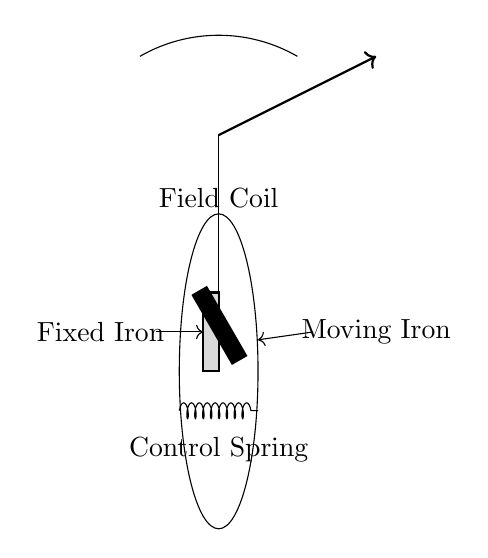
\begin{tikzpicture}
    \draw (0,0) ellipse (0.5 and 2); % Coil
    \node at (0,2.2) {Field Coil};
    
    \draw [thick, fill=gray!30] (-0.2,0) rectangle (0,1); % Fixed iron
    \node at (-1.5, 0.5) {Fixed Iron}; \draw [->] (-0.8,0.5) -- (-0.2,0.5);
    
    \draw [thick, rotate around={30:(0,0)}, fill=black] (0.2,0) rectangle (0.4,1); % Moving iron (approx)
     \node at (2, 0.5) {Moving Iron}; \draw [->] (1.2,0.5) -- (0.5,0.4);
    
    \draw [thin] (0,0) -- (0,3); % Spindle
    \draw [->, thick] (0,3) -- (2,4); % Pointer
    \draw (1,4) arc (60:120:2); % Scale
    
    \draw [decorate,decoration={coil,aspect=0.3,segment length=1mm,amplitude=1mm}] (-0.5,-0.5) -- (0.5,-0.5); % Spring
    \node at (0,-1) {Control Spring};
\end{tikzpicture}
\captionof{figure}{Repulsion Type MI Instrument}
\end{center}

\textbf{Explanation:}
\begin{itemize}
    \item Consists of a fixed coil carrying current.
    \item Two soft iron pieces: one fixed to the coil frame, one movable attached to spindle.
    \item When current flows, both irons are magnetized with same polarity.
    \item Repulsion occurs, moving the spindle and pointer.
    \item Control torque provided by spring; damping by air friction piston.
\end{itemize}
\end{solutionbox}

\begin{mnemonicbox}
\mnemonic{MIRROR: Magnetic Interaction Requires Repulsion Of Related irons}
\end{mnemonicbox}

\questionmarks{2(c OR)}{7}{Describe construction diagram of Energy meter and explain in detail.}

\begin{solutionbox}
Electronic energy meter measures kWh consumption.

\textbf{Block Diagram:}
\begin{center}
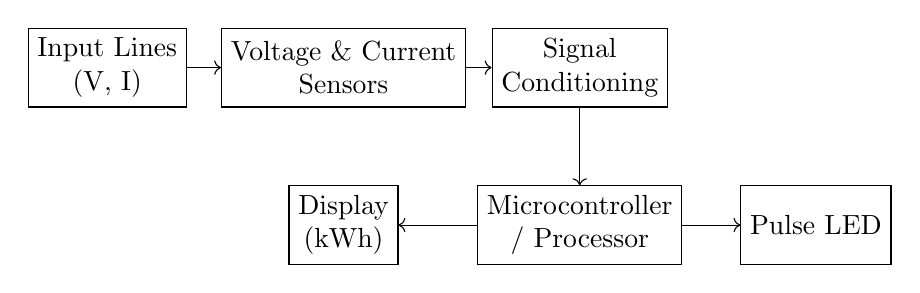
\begin{tikzpicture}[node distance=1.5cm, auto, every node/.style={rectangle, draw, align=center, minimum height=1cm}]
    \node (in) {Input Lines\\(V, I)};
    \node [right of=in, node distance=3cm] (sens) {Voltage \& Current\\Sensors};
    \node [right of=sens, node distance=3cm] (cond) {Signal\\Conditioning};
    \node [below of=cond, node distance=2cm] (proc) {Microcontroller\\/ Processor};
    \node [left of=proc, node distance=3cm] (disp) {Display\\(kWh)};
    \node [right of=proc, node distance=3cm] (led) {Pulse LED};

    \draw [->] (in) -- (sens);
    \draw [->] (sens) -- (cond);
    \draw [->] (cond) -- (proc);
    \draw [->] (proc) -- (disp);
    \draw [->] (proc) -- (led);
\end{tikzpicture}
\captionof{figure}{Electronic Energy Meter}
\end{center}

\textbf{Working:}
\begin{itemize}
    \item \textbf{Sensing}: Voltage divider and shunt/CT sense voltage and current.
    \item \textbf{Multiplication}: Instantaneous $V$ and $I$ are multiplied to get Power ($P$).
    \item \textbf{Integration}: Power is integrated over time ($\int P dt$) to get Energy.
    \item \textbf{Display}: Result is stored and shown on LCD in kWh. Pulse LED blinks proportional to consumption.
\end{itemize}
\end{solutionbox}

\begin{mnemonicbox}
\mnemonic{WATTAGE: Work And Time Tracked As Generated Electrical energy}
\end{mnemonicbox}


% ==================================================================
% QUESTION 3
% ==================================================================

\questionmarks{3(a)}{3}{Apply Lissajous pattern for frequency measurement and Phase angle measurement.}

\begin{solutionbox}
Lissajous patterns are formed on CRO X-Y mode.

\textbf{Frequency Measurement:}
\begin{itemize}
    \item $f_y / f_x = \frac{\text{Tangents on Horizontal}}{\text{Tangents on Vertical}}$
    \item Circle/Ellipse = 1:1 ratio.
    \item Figure 8 = 2:1 ratio.
\end{itemize}

\textbf{Phase Measurement (1:1 ratio):}
\begin{itemize}
    \item Pattern is an ellipse.
    \item $\sin \phi = A/B$
    \item $A$: Intercept on Y-axis (center to intersection).
    \item $B$: Max deflection on Y-axis.
    \item Circle = $90^\circ$, Line = $0^\circ$ or $180^\circ$.
\end{itemize}
\end{solutionbox}

\begin{mnemonicbox}
\mnemonic{LIPS: Lissajous Indicates Phase and Signal frequency}
\end{mnemonicbox}

\questionmarks{3(b)}{4}{Explain Graticules in CRO also Explain its types.}

\begin{solutionbox}
Graticules are the grid lines on the CRO screen for measurement.

\textbf{Types:}
\begin{center}
\captionof{table}{Types of CRO Graticules}
\begin{tabulary}{\linewidth}{|L|L|}
\hline
\textbf{Type} & \textbf{Feature} \\ \hline
\textbf{Internal} & Etched inside CRT faceplate. No parallax error. \\ \hline
\textbf{External} & Plastic sheet overlay. Cheap, easily changeable, but parallax error exists. \\ \hline
\textbf{Electronic} & Generated by electron beam. Very accurate, no parallax. \\ \hline
\end{tabulary}
\end{center}

\begin{center}
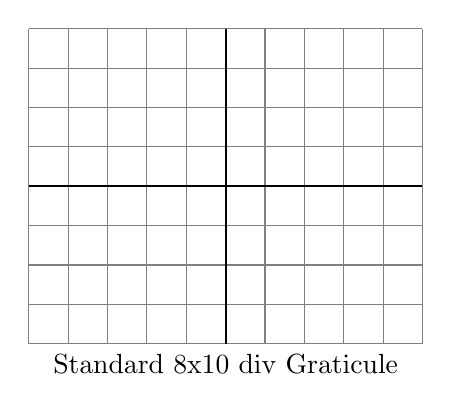
\begin{tikzpicture}[scale=0.5]
    \draw [step=1cm, gray, thin] (0,0) grid (10,8);
    \draw [thick] (5,0) -- (5,8); % Y axis
    \draw [thick] (0,4) -- (10,4); % X axis
    \node at (5,-0.5) {Standard 8x10 div Graticule};
\end{tikzpicture}
\captionof{figure}{CRO Graticule}
\end{center}
\end{solutionbox}

\begin{mnemonicbox}
\mnemonic{GRID: Graticule References for Intensity and Distance}
\end{mnemonicbox}

\questionmarks{3(c)}{7}{Describe Construction, Block diagram, working and advantage of Digital storage oscilloscope (DSO).}

\begin{solutionbox}
\textbf{Block Diagram:}
\begin{center}
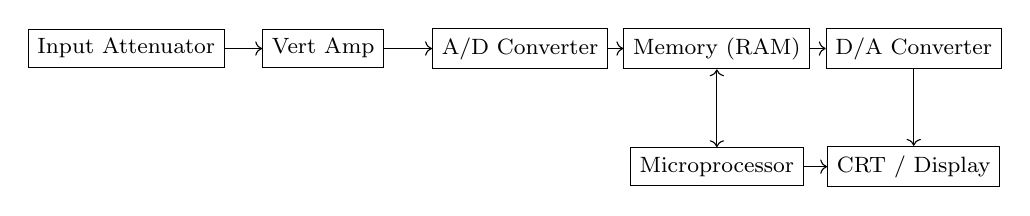
\begin{tikzpicture}[node distance=1.5cm, auto, every node/.style={rectangle, draw, align=center, font=\footnotesize}]
    \node (in) {Input Attenuator};
    \node [right of=in, node distance=2.5cm] (amp) {Vert Amp};
    \node [right of=amp, node distance=2.5cm] (adc) {A/D Converter};
    \node [right of=adc, node distance=2.5cm] (mem) {Memory (RAM)};
    \node [below of=mem] (proc) {Microprocessor};
    \node [right of=mem, node distance=2.5cm] (dac) {D/A Converter};
    \node [below of=dac] (disp) {CRT / Display};
    
    \draw [->] (in) -- (amp);
    \draw [->] (amp) -- (adc);
    \draw [->] (adc) -- (mem);
    \draw [->] (mem) -- (dac);
    \draw [->] (dac) -- (disp);
    \draw [<->] (proc) -- (mem);
    \draw [->] (proc) -- (disp);
\end{tikzpicture}
\captionof{figure}{DSO Block Diagram}
\end{center}

\textbf{Working:}
\begin{enumerate}
    \item Analog signal is sampled and digitized by ADC.
    \item Digital data stored in memory (RAM).
    \item Microprocessor processes data (measurements, math).
    \item Data converted back to analog (DAC) or directly driven to display.
\end{enumerate}

\textbf{Advantages:}
\begin{itemize}
    \item Storage of waveforms (indefinite time).
    \item Pre-trigger viewing.
    \item Capture of single-shot/transient events.
    \item Direct digital measurements (V, t, f).
    \item PC connectivity.
\end{itemize}
\end{solutionbox}

\begin{mnemonicbox}
\mnemonic{SAMPLE: Storage And Memory Processes Live Events}
\end{mnemonicbox}

\questionmarks{3(a OR)}{3}{Differentiate between CRO and DSO.}

\begin{solutionbox}
\begin{center}
\captionof{table}{Comparison: CRO vs DSO}
\begin{tabulary}{\linewidth}{|L|L|L|}
\hline
\textbf{Feature} & \textbf{CRO (Analog)} & \textbf{DSO (Digital)} \\ \hline
\textbf{Processing} & Real-time Analog & Digital sampling \\ \hline
\textbf{Storage} & None (Phosphor persistence) & Digital Memory \\ \hline
\textbf{Bandwidth} & Higher for price & Limited by Sample Rate \\ \hline
\textbf{Transients} & Cannot capture well & Easily captures \\ \hline
\textbf{Pre-trigger} & No & Yes \\ \hline
\end{tabulary}
\end{center}
\end{solutionbox}

\begin{mnemonicbox}
\mnemonic{ASPAD: Analog Shows Present; Digital Archives Data}
\end{mnemonicbox}

\questionmarks{3(b OR)}{4}{Explain structure of 10:1 Probes in detail.}

\begin{solutionbox}
10:1 probe attenuates signal by factor of 10 to increase input impedance and reduce loading.

\textbf{Structure:}
\begin{center}
\begin{circuitikz}[auto]
    \node [left] at (0,2) {Tip};
    \draw (0,2) to [R, l=$R_p (9M\Omega)$] (3,2);
    \draw (0.5,2) -- (0.5,3) to [C, l=$C_p (Comp)$] (2.5,3) -- (2.5,2); % tuning cap in parallel
    
    \draw (3,2) -- (5,2) node[right] {To Scope ($1M\Omega$)};
    \draw (3,2) to [C, l=$C_{cable}$] (3,0) node[ground]{};
    \node at (4,1) {Cable};
\end{circuitikz}
\captionof{figure}{10:1 Probe Circuit}
\end{center}

\textbf{Details:}
\begin{itemize}
    \item Contains a 9 M$\Omega$ resistor in series with the scope's 1 M$\Omega$ input.
    \item Total resistance = 10 M$\Omega$. Voltage division ratio = 10:1.
    \item Adjustable capacitor compensates for cable capacitance to ensure flat frequency response.
\end{itemize}
\end{solutionbox}

\begin{mnemonicbox}
\mnemonic{TAPER: Ten-to-one Attenuation Preserves and Extends Range}
\end{mnemonicbox}

\questionmarks{3(c OR)}{7}{Describe Block diagram, working and application of CRO.}

\begin{solutionbox}
\textbf{Block Diagram:}
\begin{center}
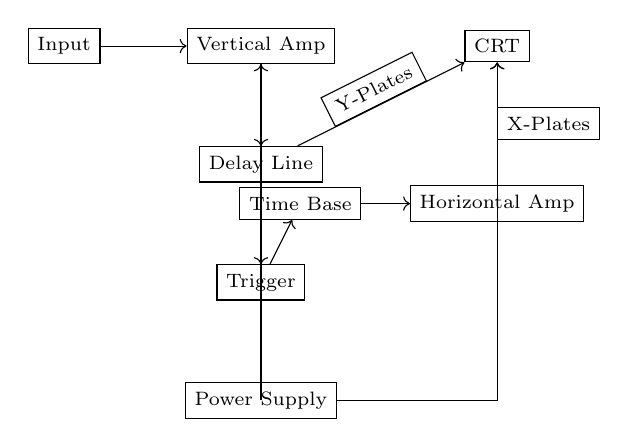
\begin{tikzpicture}[auto, node distance=1.5cm, every node/.style={rectangle, draw, align=center, font=\scriptsize}]
    \node (crt) {CRT};
    \node [left of=crt, node distance=3cm] (va) {Vertical Amp};
    \node [below of=crt, node distance=2cm] (ha) {Horizontal Amp};
    \node [below of=va] (dl) {Delay Line};
    \node [left of=va, node distance=2.5cm] (in) {Input};
    \node [below of=dl] (trig) {Trigger};
    \node [left of=ha, node distance=2.5cm] (tb) {Time Base};
    \node [below of=trig] (ps) {Power Supply};
    
    \draw [->] (in) -- (va);
    \draw [->] (va) -- (dl);
    \draw [->] (dl) -- node[above, sloped] {Y-Plates} (crt);
    \draw [->] (va) -- (trig);
    \draw [->] (trig) -- (tb);
    \draw [->] (tb) -- (ha);
    \draw [->] (ha) -- node[right] {X-Plates} (crt);
    \draw [->] (ps) -| (crt);
    \draw [->] (ps) -| (va);
\end{tikzpicture}
\captionof{figure}{CRO Block Diagram}
\end{center}

\textbf{Working:}
\begin{itemize}
    \item \textbf{Vertical System}: Amplifies signal for Y-deflection.
    \item \textbf{Horizontal System}: Generates sawtooth wave (Time Base) for X-sweep.
    \item \textbf{Trigger}: Synchronizes sweep with signal start.
    \item \textbf{CRT}: Displays the trace.
\end{itemize}

\textbf{Applications:} Voltage, frequency, phase measurement, waveform observation.
\end{solutionbox}

\begin{mnemonicbox}
\mnemonic{VIEW: Voltage Inspection and Electrical Waveform observation}
\end{mnemonicbox}


% ==================================================================
% QUESTION 4
% ==================================================================

\questionmarks{4(a)}{3}{Differentiate RTD and Thermistor.}

\begin{solutionbox}
\begin{center}
\captionof{table}{Comparison: RTD vs Thermistor}
\begin{tabulary}{\linewidth}{|L|L|L|}
\hline
\textbf{Parameter} & \textbf{RTD} & \textbf{Thermistor} \\ \hline
\textbf{Material} & Pure Metal (Pt, Ni) & Semiconductor \\ \hline
\textbf{Coeff ($ \alpha $)} & Positive (PTC) & Usually Negative (NTC) \\ \hline
\textbf{Linearity} & Linear & Highly Non-linear \\ \hline
\textbf{Range} & Wide ($-200^\circ$C to $850^\circ$C) & Medium ($-50^\circ$C to $300^\circ$C) \\ \hline
\textbf{Sensitivity} & Low ($0.4\%/^\circ$C) & High ($4\%/^\circ$C) \\ \hline
\end{tabulary}
\end{center}
\end{solutionbox}

\begin{mnemonicbox}
\mnemonic{METAL-SEMI: Metal Linear vs Semi Non-linear}
\end{mnemonicbox}

\questionmarks{4(b)}{4}{Give and explain two example of primary and Secondary transducer.}

\begin{solutionbox}
\begin{center}
\captionof{table}{Primary vs Secondary Transducers}
\begin{tabulary}{\linewidth}{|L|L|}
\hline
\textbf{Primary Transducer} & \textbf{Secondary Transducer} \\ \hline
\textbf{Thermocouple}: Converts temp directly to voltage. & \textbf{LVDT}: Converts displacement to voltage (requires excitation). \\ \hline
\textbf{Piezoelectric}: Converts force directly to charge. & \textbf{Strain Gauge}: Resistance changes with strain (needs bridge to read voltage). \\ \hline
\end{tabulary}
\end{center}
\textbf{Explanation}:
\begin{itemize}
    \item \textbf{Primary}: Direct conversion from physical to electrical quantity.
    \item \textbf{Secondary}: Requires an intermediate stage or external power to produce electrical signal.
\end{itemize}
\end{solutionbox}

\begin{mnemonicbox}
\mnemonic{PIDS: Primary Is Direct; Secondary is Stepwise}
\end{mnemonicbox}

\questionmarks{4(c)}{7}{Describe Thermocouple with working principle, types and application.}

\begin{solutionbox}
\textbf{Principle (Seebeck Effect):} When two dissimilar metals are joined at two junctions kept at different temperatures, an EMF is generated proportional to the temperature difference.

\textbf{Construction:}
\begin{center}
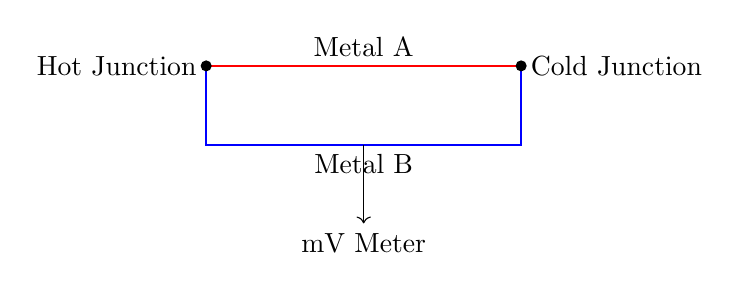
\begin{tikzpicture}
    \draw [thick, red] (0,0) -- (4,0); \node [above] at (2,0) {Metal A};
    \draw [thick, blue] (0,0) -- (0,-1) -- (2,-1) -- (4,-1) -- (4,0); \node [below] at (2,-1) {Metal B};
    \fill (0,0) circle (2pt) node[left] {Hot Junction};
    \fill (4,0) circle (2pt) node[right] {Cold Junction};
    \draw [->] (2,-1) -- (2,-2) node [below] {mV Meter};
\end{tikzpicture}
\captionof{figure}{Thermocouple}
\end{center}

\textbf{Types:}
\begin{itemize}
    \item \textbf{Type J}: Iron-Constantan ($-40$ to $750^\circ$C)
    \item \textbf{Type K}: Chromel-Alumel ($-200$ to $1350^\circ$C) - Most common.
    \item \textbf{Type T}: Copper-Constantan (Low temp).
    \item \textbf{Type R/S}: Platinum-Rhodium (High temp/Precision).
\end{itemize}

\textbf{Applications:} Furnaces, Gas turbines, Engines, Industrial temp monitoring.
\end{solutionbox}

\begin{mnemonicbox}
\mnemonic{STEVE: Seebeck Thermoelectric Effect Verifies Elevated temperatures}
\end{mnemonicbox}

\questionmarks{4(a OR)}{3}{Demonstrate working and principle Semiconductor Temperature Sensor LM35.}

\begin{solutionbox}
\textbf{Principle:} Integrated circuit sensor where output voltage is linearly proportional to Centigrade temperature ($10$ mV/$^\circ$C).

\textbf{Features:}
\begin{itemize}
    \item Calibrated directly in Celsius.
    \item Linear +$10.0$ mV/$^\circ$C scale factor.
    \item Range: $-55^\circ$ to $+150^\circ$C.
\end{itemize}

\begin{center}
\begin{circuitikz}[auto]
    \node [draw, rectangle, minimum width=1.5cm, minimum height=2cm] (ic) {LM35};
    \draw (ic.west) -- ++(-1,0) node[left] {$+V_s$ (4-20V)};
    \draw (ic.east) -- ++(1,0) node[right] {$V_{out}$};
    \draw (ic.south) -- ++(0,-1) node[ground]{};
\end{circuitikz}
\captionof{figure}{LM35 Connection}
\end{center}
\end{solutionbox}

\begin{mnemonicbox}
\mnemonic{LOTUS: Linear Output Temperature Units from Semiconductor}
\end{mnemonicbox}

\questionmarks{4(b OR)}{4}{Describe incremental type of Optical encoder with it's output waveform.}

\begin{solutionbox}
Optical encoder measures position/speed using light pulses.

\textbf{Construction:}
\begin{itemize}
    \item Rotating disk with slots.
    \item LED source and Photodetector.
    \item As disk rotates, beam is interrupted, generating pulses.
\end{itemize}

\textbf{Output Waveform:}
\begin{center}
\begin{tikzpicture}
    \draw [->] (0,0) -- (6,0) node[right] {Time};
    \draw [->] (0,0) -- (0,3) node[above] {Amp};
    
    % Channel A
    \draw [thick, blue] (0,2) -- (1,2) -- (1,2.8) -- (2,2.8) -- (2,2) -- (3,2) -- (3,2.8) -- (4,2.8) -- (4,2);
    \node [left] at (0,2.4) {Ch A};
    
    % Channel B (Quadrature)
    \draw [thick, red] (0,0.5) -- (0.5,0.5) -- (0.5,1.3) -- (1.5,1.3) -- (1.5,0.5) -- (2.5,0.5) -- (2.5,1.3) -- (3.5,1.3) -- (3.5,0.5);
    \node [left] at (0,0.9) {Ch B};
\end{tikzpicture}
\captionof{figure}{Quadrature Output}
\end{center}
Offset allows direction detection.
\end{solutionbox}

\begin{mnemonicbox}
\mnemonic{PADS: Pulses from A and Determine Speed}
\end{mnemonicbox}

\questionmarks{4(c OR)}{7}{Describe construction, operation of LVDT with advantages, disadvantages and application.}

\begin{solutionbox}
LVDT (Linear Variable Differential Transformer) measures linear displacement.

\textbf{Construction:}
\begin{center}
\begin{circuitikz}[auto]
    \draw (0,0) to [L, l=Pri] (0,2);
    \draw (2,2.5) to [L, l=$Sec_1$] (2,1.5);
    \draw (2,0.5) to [L, l=$Sec_2$] (2,-0.5);
    \draw [thick] (0.8,-0.5) rectangle (1.2, 2.5); \node at (1,3) {Core};
    \draw [->] (1, 1) -- (1, 1.5); \draw [->] (1, 1) -- (1, 0.5); % Motion
\end{circuitikz}
\captionof{figure}{LVDT Schematic}
\end{center}

\textbf{Operation:} AC applied to Primary. Core position varies flux linkage to Secondaries ($S_1, S_2$). Output $V_{out} = V_{s1} - V_{s2}$. Null at center.

\textbf{Pros}: Frictionless, infinite resolution, robust.\\
\textbf{Cons}: AC required, temp sensitive.\\
\textbf{App}: Displacement, pressure measurement.
\end{solutionbox}

\begin{mnemonicbox}
\mnemonic{MOVE-AC: Magnetic Output Varies with Exact Armature Core}
\end{mnemonicbox}


% ==================================================================
% QUESTION 5
% ==================================================================

\questionmarks{5(a)}{3}{Describe working of Pressure measurement using Capacitive transducer.}

\begin{solutionbox}
\textbf{Principle:} Pressure deforms a diaphragm, changing the distance ($d$) between capacitor plates, thus changing capacitance ($C \propto 1/d$).

\begin{center}
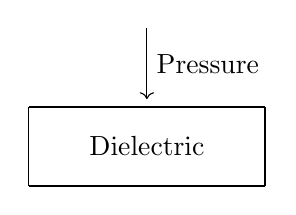
\begin{tikzpicture}
    \draw [thick] (0,0) -- (3,0); % Fixed plate
    \draw [thick] (0,1) -- (3,1); % Diaphragm
    \draw [->] (1.5, 2) -- (1.5, 1.1) node [midway, right] {Pressure};
    \draw (0,0) -- (0,1); \draw (3,0) -- (3,1); % Housing
    \node at (1.5, 0.5) {Dielectric};
\end{tikzpicture}
\captionof{figure}{Capacitive Pressure Sensor}
\end{center}
\end{solutionbox}

\begin{mnemonicbox}
\mnemonic{CAPS: Capacitance Alters as Pressure Shifts}
\end{mnemonicbox}

\questionmarks{5(b)}{4}{Define rise time, fall time, Pulse width and duty cycle.}

\begin{solutionbox}
\begin{center}
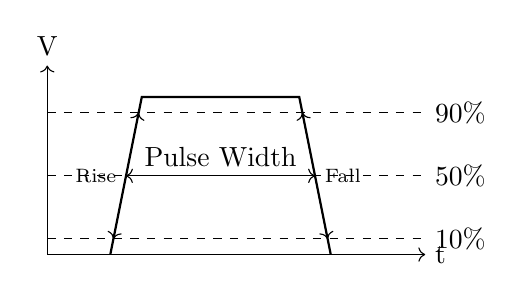
\begin{tikzpicture}[scale=0.8]
    \draw [->] (0,0) -- (6,0) node[right] {t};
    \draw [->] (0,0) -- (0,3) node[above] {V};
    
    \draw [thick] (1,0) -- (1.5,2.5) -- (4,2.5) -- (4.5,0);
    \draw [dashed] (0,0.25) -- (6,0.25) node[right] {10\%};
    \draw [dashed] (0,2.25) -- (6,2.25) node[right] {90\%};
    \draw [dashed] (0,1.25) -- (6,1.25) node[right] {50\%};
    
    \draw [<->] (1.05,0.25) -- (1.45,2.25) node[midway, left] {\scriptsize Rise};
    \draw [<->] (4.05,2.25) -- (4.45,0.25) node[midway, right] {\scriptsize Fall};
    \draw [<->] (1.25,1.25) -- (4.25,1.25) node[midway, above] {Pulse Width};
\end{tikzpicture}
\captionof{figure}{Pulse Characteristics}
\end{center}
\begin{itemize}
    \item \textbf{Rise Time}: 10\% to 90\% of max.
    \item \textbf{Fall Time}: 90\% to 10\% of max.
    \item \textbf{Pulse Width}: Width at 50\%.
    \item \textbf{Duty Cycle}: (Pulse Width / Total Period) $\times 100\%$.
\end{itemize}
\end{solutionbox}

\begin{mnemonicbox}
\mnemonic{RPFD: Rise Pulses, Fall Determines}
\end{mnemonicbox}

\questionmarks{5(c)}{7}{Discuss Function generator block diagram.}

\begin{solutionbox}
Produces Sine, Square, Triangle waves.

\textbf{Block Diagram:}
\begin{center}
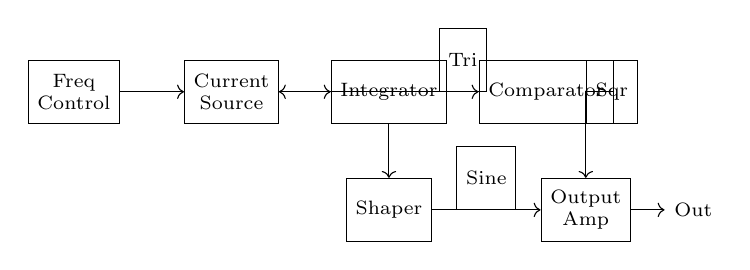
\begin{tikzpicture}[node distance=1.5cm, auto, every node/.style={rectangle, draw, align=center, font=\scriptsize, minimum height=0.8cm}]
    \node (freq) {Freq\\Control};
    \node [right of=freq, node distance=2cm] (src) {Current\\Source};
    \node [right of=src, node distance=2cm] (int) {Integrator};
    \node [right of=int, node distance=2cm] (comp) {Comparator};
    \node [below of=int] (shape) {Shaper};
    \node [right of=shape, node distance=2.5cm] (amp) {Output\\Amp};
    
    \draw [->] (freq) -- (src);
    \draw [->] (src) -- (int);
    \draw [->] (int) -- node[above] {Tri} (comp);
    \draw [->] (comp) -- (src); % Feedback
    \draw [->] (comp) -| node[right] {Sqr} (amp);
    \draw [->] (int) -- (shape);
    \draw [->] (shape) -- node[above] {Sine} (amp);
    \draw [->] (amp) -- ++(1,0) node[right, draw=none] {Out};
\end{tikzpicture}
\captionof{figure}{Function Generator}
\end{center}

\textbf{Working:}
\begin{itemize}
    \item Integrator + Comparator loop generates Triangle and Square.
    \item Sine shaper (diode network) converts Triangle to Sine.
    \item Output amplifier adjusts Amplitude and Offset.
\end{itemize}
\end{solutionbox}

\begin{mnemonicbox}
\mnemonic{FASTEST: Frequency Amplitude Shaping Together Ensures Signal Types}
\end{mnemonicbox}

\questionmarks{5(a OR)}{3}{Discuss Working, construction of strain gauge.}

\begin{solutionbox}
\textbf{Construction:} Fine wire grid on backing material.
\textbf{Working:}
\begin{itemize}
    \item Bonded to test object.
    \item Deformation changes length ($l$) and area ($A$), changing resistance $R = \rho l / A$.
    \item $\Delta R/R = G \times \epsilon$ (G = Gauge Factor, $\epsilon$ = Strain).
\end{itemize}
\end{solutionbox}

\begin{mnemonicbox}
\mnemonic{SERB: Strain Effects Resistance by Bonding}
\end{mnemonicbox}

\questionmarks{5(b OR)}{4}{Describe working of Digital IC tester with suitable diagrams.}

\begin{solutionbox}
Tests logic gates/ICs by applying truth table inputs and complying outputs.

\textbf{Block Diagram:}
\begin{center}
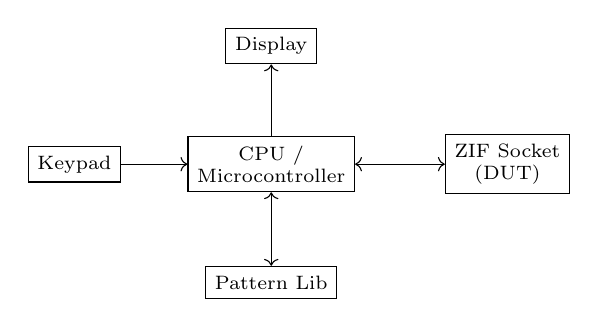
\begin{tikzpicture}[node distance=1.5cm, auto, every node/.style={rectangle, draw, align=center, font=\scriptsize}]
    \node (cpu) {CPU /\\Microcontroller};
    \node [left of=cpu, node distance=2.5cm] (key) {Keypad};
    \node [above of=cpu] (disp) {Display};
    \node [right of=cpu, node distance=3cm] (sock) {ZIF Socket\\(DUT)};
    \node [below of=cpu] (lib) {Pattern Lib};
    
    \draw [->] (key) -- (cpu);
    \draw [->] (cpu) -- (disp);
    \draw [<->] (cpu) -- (sock);
    \draw [<->] (cpu) -- (lib);
\end{tikzpicture}
\captionof{figure}{IC Tester}
\end{center}

\textbf{Working:}
\begin{enumerate}
    \item Select IC number.
    \item CPU fetches test patterns from library.
    \item Applies inputs to DUT pins.
    \item Reads outputs and compares with expected.
    \item Displays Pass/Fail.
\end{enumerate}
\end{solutionbox}

\begin{mnemonicbox}
\mnemonic{PIPE: Pattern Input, Pin Examination}
\end{mnemonicbox}

\questionmarks{5(c OR)}{7}{Discuss working of Spectrum Analyzer with suitable diagrams.}

\begin{solutionbox}
Displays Amplitude vs Frequency.

\textbf{Block Diagram (Swept Superheterodyne):}
\begin{center}
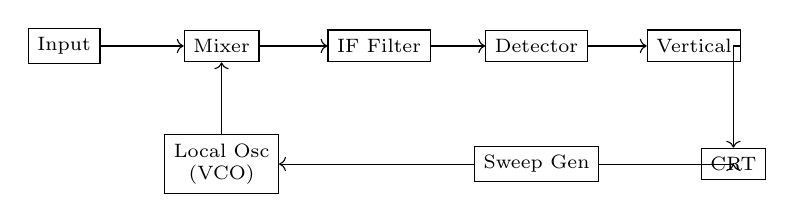
\begin{tikzpicture}[node distance=1.5cm, auto, every node/.style={rectangle, draw, align=center, font=\scriptsize}]
    \node (in) {Input};
    \node [right of=in, node distance=2cm] (mix) {Mixer};
    \node [right of=mix, node distance=2cm] (if) {IF Filter};
    \node [right of=if, node distance=2cm] (det) {Detector};
    \node [right of=det, node distance=2cm] (vert) {Vertical};
    \node [below of=mix] (lo) {Local Osc\\(VCO)};
    \node [below of=det] (sweep) {Sweep Gen};
    \node [right of=sweep, node distance=2.5cm] (crt) {CRT};
    
    \draw [->] (in) -- (mix);
    \draw [->] (mix) -- (if);
    \draw [->] (if) -- (det);
    \draw [->] (det) -- (vert);
    \draw [->] (vert) -| (crt);
    \draw [->] (lo) -- (mix);
    \draw [->] (sweep) -- (lo);
    \draw [->] (sweep) -| (crt);
\end{tikzpicture}
\captionof{figure}{Spectrum Analyzer}
\end{center}

\textbf{Working:}
\begin{itemize}
    \item Sweep generator ramps LO frequency and drives X-axis.
    \item Mixer shifts input frequencies to IF.
    \item IF filter selects current frequency component.
    \item Detector recovers amplitude (Y-axis).
\end{itemize}
\end{solutionbox}

\begin{mnemonicbox}
\mnemonic{SHAFT: Sweep, Heterodyne, Analyze Frequency and Time}
\end{mnemonicbox}

\end{document}
